\section{Experimental Evaluation} % 70/300 points, 23%

We fine-tune and evaluate the \BertSumAbs summarization model from the reproduced paper by \citeauthor{LiuL2019} on a A100 GPU using the Flux framework on Julia~\cite{InnesSFGRJKPS2018,BezansonEKS2017,LiuL2019}.
A scaled-down variant of their \TransformerAbs model, that we call \TransformerAbsTiny, is trained from scratch on a GeForce MX150 GPU for testing our evaluation workflow.
We train both models using the CNN/Daily Mail datasets, but use the preprocessed variant by \citeauthor{LiuL2019} instead of the original data by \citeauthor{HermannKGEKSB2015}~\cite{LiuL2019,HermannKGEKSB2015}.
Our implementation resembles the same encoder-decoder architecture as used by \citeauthor{LiuL2019}, uses the same \BertBase model for the pretrained encoder, and \Bert's WordPiece tokenizer to transform raw text into embeddable tokens~\cite{LiuL2019,DevlinCLT2019}.
Though, we do not tune any hyperparameters of either the model or the optimizers.
We also reimplement the beam search algorithm.
Due to instabilities in fine-tuning and hardware constraints we were unable to train the model for the full 200\,000 steps proposed by \citeauthor{LiuL2019}~\cite{LiuL2019}.
We assume that the complex hyperparameter settings and large model size used in their paper are prone to fine-tuning issues like we experienced, a problem that has only recently gained more attention~\cite{DodgeISFHS2020,ZhangWKWA2020,AghajanyanSGGZG2020}.

\subsection{Dataset}

We train and evaluate the summarization model on the CNN/Daily Mail benchmark dataset using the standard training, test, and validation splits, as crawled by \citeauthor{NallapatiZSGX2016}~\cite{HermannKGEKSB2015,NallapatiZSGX2016}.
\citeauthor{LiuL2019} preprocess the raw non-anomized CNN/Daily Mail dataset, split sentences with the Stanford CoreNLP framework~\cite{ManningSBFBM2014}, and release the preprocessed data publicly~\cite{LiuL2019}.
Our implementation is designed to automatically download those preprocessed CNN/Daily Mail datasets from the Web\footnote{\url{https://drive.google.com/open?id=1DN7ClZCCXsk2KegmC6t4ClBwtAf5galI}}, no manual downloads are needed.

Even though \citeauthor{LiuL2019} claim to truncate input sequences after 512 tokens, we observe sequences longer than 512 tokens in the preprocessed data~\cite{LiuL2019}.
We use the opportunity to not truncate input sequences, because we find that truncating after only 512 tokens discards a reasonable amount~(33\,\% on average) of context from the news articles~\cite{NallapatiZSGX2016}.\footnote{Arguably, especially the last sentences of a news article can be important to draw the right conclusion in a summary.}
From the preprocessed data we extract pairs of each source article with its target summary, normalize sentence separators, and tokenize with \Bert's \WordPiece tokenizer~\cite{DevlinCLT2019}.

Like \citeauthor{LiuL2019}, we use the \BertBase model, pretrained by \citeauthor{DevlinCLT2019}, as encoder~\cite{DevlinCLT2019}.
That \Bert model is also automtically downloaded from the Web along with its \WordPiece tokenizer.\footnote{\Bert is loaded by the Transformers library: \url{https://github.com/chengchingwen/Transformers.jl}}

\subsection{Abstractive Summarizaion Model}

Our implementation of the \BertSumAbs abstractive summarization model follows the same encoder-decoder architecture as described by \citeauthor{LiuL2019}~\cite{LiuL2019}.
Input and output tokens are embedded with learned word embeddings and position embeddings with a max length of 4096~tokens.
Our transformer decoder is made of 6~transformer layers that each have 768~hidden units with a hidden size of~2048 for feed-forward layers.
We apply dropout with a probability of 0.1 before all linear layers, the same parameters as used by \citeauthor{LiuL2019}~\cite{LiuL2019}.
A linear layer with softmax activation function generates word probabilities for the 30K tokens in \Bert's vocabulary~\cite{DevlinCLT2019}.
The full \BertSumAbs model contains 182M~trainable parameters: 27M~for embeddings, 85M~for the encoder's transformer layers, 47M~for the decoder's transformer layers, and 23M~for the generator layer.

We contrast the large \BertSumAbs with a smaller, non-pretrained baseline variant, \TransformerAbsTiny, that is designed similar to the \TransformerAbs model by \citeauthor{LiuL2019} but with even less parameters~\cite{LiuL2019}: The randomly initialized model uses 2~transformer layers for the encoder and 2~transformer layers for the decoder. All layers have only 8~hidden units with a hidden size of~4 and dropout probability 0.1.
The \TransformerAbsTiny is designed to be trainable even on low-performance machines as it only contains 37K trainable parameters.

\subsection{Fine-tuning the pretrained model}

Following the implementation of \cite{LiuL2019}, we planned to fine-tune the \BertSumAbs model for 200\,000 steps, but with gradient accumulation after each step~\cite{LiuL2019}. We save snapshots of the model, its weights, and its optimizers every 2500 steps.
Like \citeauthor{LiuL2019}, we implement a custom training schedule with separate learning rates for the pretrained encoder~(\(\eta_E\)) and randomly initialized decoder~(\(\eta_D\)):
\begin{align*}
    \eta_E &= 2e^{-3} \cdot \min( \text{step}^{-0.5},\ \text{step} \cdot 20\,000^{-1.5} ) \\
    \eta_D &= 0.1 \cdot \min( \text{step}^{-0.5},\ \text{step} \cdot 10\,000^{-1.5} )
\end{align*}
Both encoder and decoder are trained using Adam optimizers with the above learning rates, \(\beta_1 = 0.9\)~and~\(\beta_2 = 0.999\).
Cross entropy between the token probabilities predicted by the model and the observed, one-hot ground truth probabilities is used as classification loss for training the models. We do not apply label-smoothing like \citeauthor{LiuL2019} do~\cite{LiuL2019}.

Unfortunately, on our hardware (using an A100 GPU) we were unable to train the model for the full 200\,000 steps but instead had to cancel training after 22\,500 steps.
\begin{figure}
    \centering
    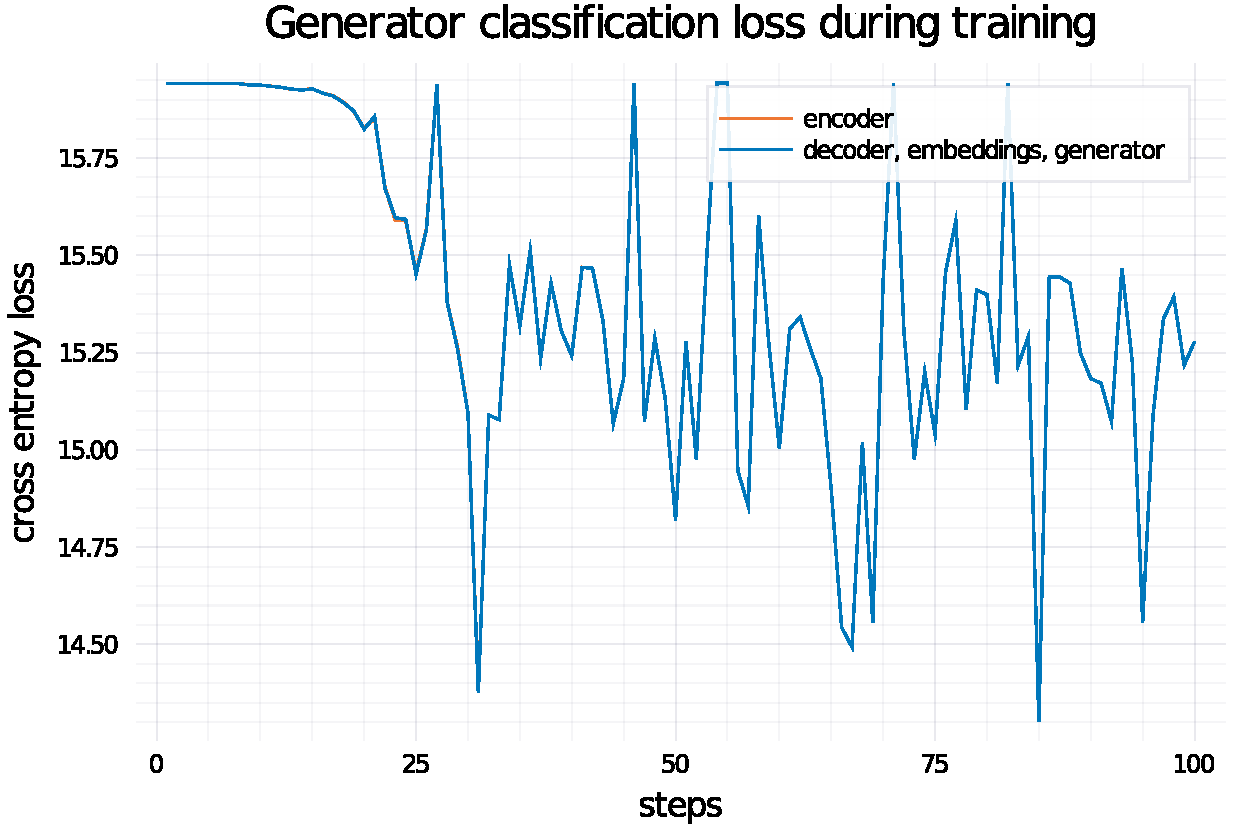
\includegraphics[width=0.7\linewidth]{training-loss-bert-abs-100.pdf}
    \caption{Cross entropy between predicted token probabilities and ground truth labels for the first 100 training steps of training the \BertSumAbs model.}
    \label{training-loss-bert-abs}
\end{figure}

Figure~\ref{training-loss-bert-abs} shows that the loss when training \BertSumAbs quickly begins to oscillate after ony 25 steps. The oscillation continues to the end of training.
\citeauthor{ZhangWKWA2020} suggest that changes in the optimizer can in some cases cause instabilities in the fine-tuning process~\cite{ZhangWKWA2020}.
Given that the \Bert encoder and transformer decoder of the \BertSumAbs model are trained with custom learning rates and Adam optimizers, we ask whether these complex hyperparameter settings are causing the observed fine-tuning issues.
A more detailed analysis has to be conducted to test if the issues can be circumvented by training with different random seeds~\cite{DodgeISFHS2020}.
New approaches also fine-tuning pretrained language models for abstractive summarization suggest an improvement by using trust regions~\cite{AghajanyanSGGZG2020}.
It is also notable that training the \BertSumAbs model on the A100 GPU used about 40GB of memory at a speed of about 9 steps per minute.
Though the memory usage is comparable to the memory usage reported by \citeauthor{LiuL2019}~\cite{LiuL2019}.
\begin{figure}
    \centering
    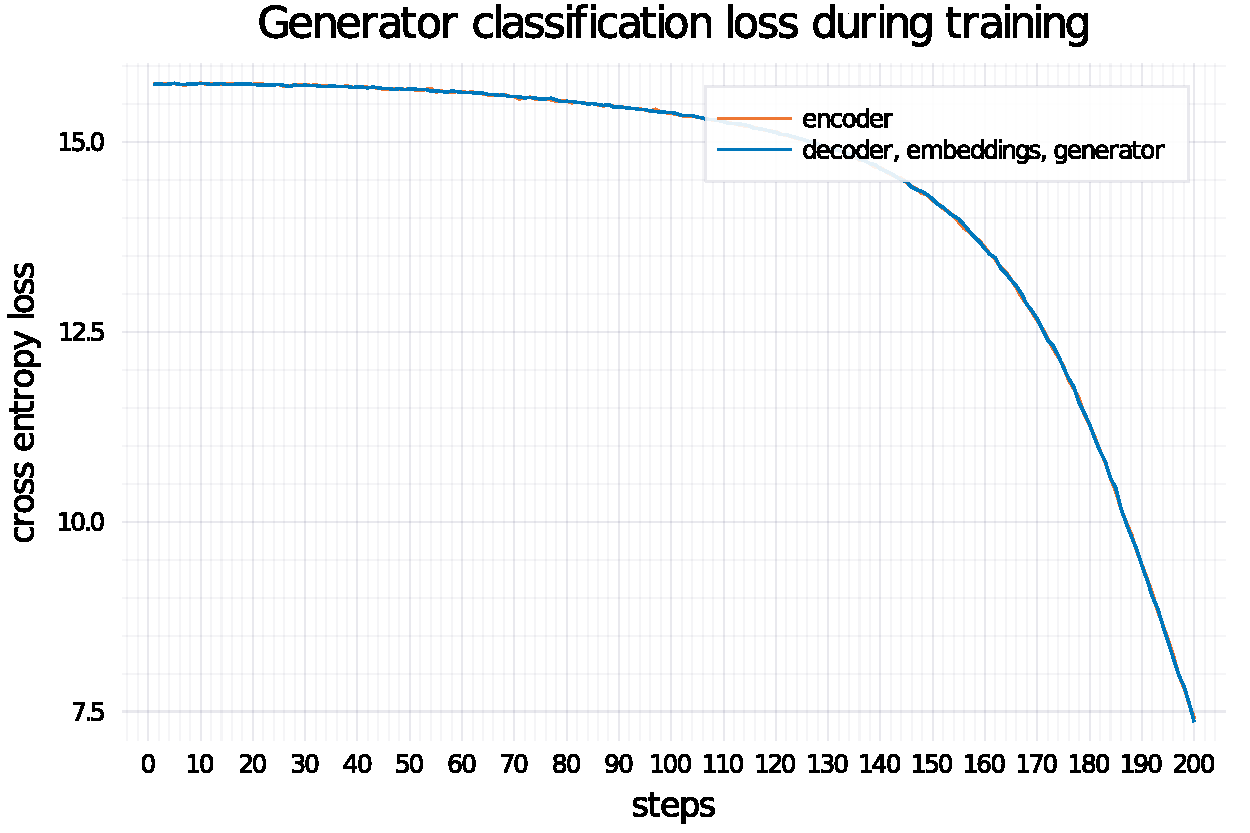
\includegraphics[width=0.7\linewidth]{training-loss-transformer-abs-tiny.pdf}
    \caption{Cross entropy between predicted token probabilities and ground truth labels for the first 200 training steps of training the \TransformerAbsTiny model.}
    \label{training-loss-transformer-abs}
\end{figure}

The small \TransformerAbsTiny model was only trained on the less powerful GeForce MX150 GPU for the first 200 training steps, but as shown in Figure~\ref{training-loss-transformer-abs}, the loss decreases more stable than for the \BertSumAbs model.

\subsection{Beam Search}

In addition to the transformer encoder-decoder model, we also reimplement the beam search algorithm with parameters used by \citeauthor{LiuL2019}.
In each iteration of the beam search algorithm we keep track of the best \(n\)~sequences based on a scoring function~\(s\).
Here, \(n\)~denotes the beam width and \(s\)~is based on the probability~\(p(x_1,\ldots,x_n)\) of each sequence~\(\mathbf{x} = [x_1,\ldots,x_n]\).
We start with the a sequence only containing the start token and then subsequently expand with new tokens from the vocabulary, until we either see the end-of-sequence token or hit a configurable maximum length.
The probability for a new sequence \(\mathbf{\hat x} = [x_1,\ldots,x_{n+1}]\) with the new token \(x_{n+1}\) is then calculated as the conditional probability
\[ p(x_1,\ldots,x_{n+1}) = p(x_{n+1}|x_1,\ldots,x_n)p(x_1,\ldots,x_n) \]
where we get the next-token prediction~\( p(x_{n+1}|x_1,\ldots,x_n) \) from the model's generator layer.
The scoring function~\(s\) is used to model maximum length~\(n_\text{max}\), length penalization with factor~\(\alpha_L\)~\cite{WuSCLNMKCGMKSJL2016}, and to block repeated trigrams~\cite{PaulusXS2018}:
\begin{align*}
    s(x_1,\ldots,x_n) = \begin{cases}
        0 & \text{if} n > n_\text{max} \\
        0 & \text{if \([x_{n-2},x_{n-1},x_n]\) occurs} \\
        & \quad\text{before in  \([x_1,\ldots,x_n]\)} \\
        p(x_1,\ldots,x_n) / \frac{(5 + n)^{\alpha_L}}{(5 + 1)^{\alpha_L}} & \text{else}
    \end{cases}
\end{align*}
Even though we were unable to test the beam search implementation as we lack a trained model for computing~\( p(x_{n+1}|x_1,\ldots,x_n) \), we confirm that on a untrained model random nonsense sequences of arbitrary length are generated that all have very low probability.

\subsection{Summary Quality}

Due to not having a trained model, we are unable to automatically or manually assess summary quality for the \BertSumAbs model.
We originally planned to automatically measure unigram overlap~(\RougeN{1}) and bigram overlap~(\RougeN{2}) between generated and ground truth summaries to assess informativeness as well as the longest common subsequence~(\RougeL) to assess fluency in terms of the \Rouge framework~\cite{Lin2004}.
\begin{table}
    \centering
    \caption{Quality labels used by human annotators to assess summary quality.}
    \label{quality-levels}
    \begin{tabular}{cl}
        \toprule
        Label & Description \\
        \midrule
        0 & unreadable summary or unrelated to original article \\
        1 & readable and related to original article, some redundancy \\
        2 & captures exactly the article's main points, no redundancy \\
        \bottomrule
    \end{tabular}
\end{table}
Additionally we planned to randomly select a small subset of generated summaries to be judged by human annotators in the three quality levels shown in Table~\ref{quality-levels}.
Though, as we are unable to evaluate summary quality without being able to train the summarization model, we cannot argue whether the \Rouge scores reported by \citeauthor{LiuL2019} could be reproduced or not~\cite{LiuL2019}.
